\chapter{Estado del arte}

{\color{blue}

Antes de empezar a desarrollar los objetivos del proyecto es necesario conocer primero los fundamentos del Internet de las Cosas, esto engloba desde su funcionamiento, tipos de arquitecturas hasta los distintos estándares que existen.

\section{Internet de las Cosas}

El término ``Internet de las Cosas`` (IoT) se conoce desde hace unos años. En los últimos tiempos, está recibiendo más atención debido al avance de la tecnología inalámbrica. La idea básica se debe a la variedad de objetos, como RFID, NFC, sensores, actuadores, teléfonos móviles, que pueden interactuar entre sí teniendo una dirección distinta. El IoT permite a los objetos ver, oír, pensar y realizar trabajos haciendo que `hablen` entre sí, para compartir y sincronizar información. El IoT transforma estos objetos de convencionales a inteligentes mediante la manipulación de sus tecnologías subyacentes, como los dispositivos integrados, las tecnologías de comunicación, las redes de sensores, los protocolos y las aplicaciones. \cite{7589556} \\

La premisa básica y el objetivo de IoT es ``conectar lo que no está conectado``. Esto significa que los objetos que no están actualmente unidos a una red informática, es decir, a Internet, se conectarán para que puedan comunicarse e interactuar con personas y otros objetos. IoT es una transición tecnológica en la que los dispositivos nos permitirán sentir y controlar el mundo físico haciendo que los objetos sean más inteligentes y conectándolos a través de una red inteligente. Cuando los objetos y las máquinas pueden ser detectados y controlados a distancia a través de una red, se consigue una mayor integración entre el mundo físico y los ordenadores. Esto permite mejoras en las áreas de eficiencia, precisión, automatización y habilitación de aplicaciones avanzadas. \\

El mundo del IoT es amplio y puede resultar algo complicado al principio debido a la abundancia de componentes y protocolos que engloba. En lugar de considerar IoT como un único tecnología, es bueno verlo como un paraguas de varios conceptos, protocolos y tecnologías, todos ellos dependientes a veces de un sector concreto. Aunque la amplia gama de elementos de IoT está diseñado para crear numerosos beneficios en las áreas de productividad y automatización, al mismo al mismo tiempo, introduce nuevos retos, como la ampliación del gran número de dispositivos y de la cantidad de datos que deben procesarse. \cite{hanes2017iot}

\subsection{Arquitecturas}

En esta sección se muestran distintas arquitecturas para el IoT, que suele describirse como un proceso de cuatro etapas en el que los datos fluyen desde los sensores conectados a las "cosas" a través de una red y, finalmente, a un centro de datos corporativo o a la nube para su procesamiento, análisis y almacenamiento.

\subsubsection{Arquitectura de tres capas}

Normalmente, la arquitectura de IoT se divide en tres capas básicas: capa de aplicación, capa de red y capa de percepción, que se describen con más detalle a continuación.

\begin{itemize}
    \item \textbf{Capa de percepción.} También conocida como capa de sensores, se implementa como la capa inferior en la arquitectura de IoT. La capa de percepción interactúa con los dispositivos y componentes físicos a través de dispositivos inteligentes (RFID, sensores, actuadores, etc.). Sus principales objetivos son conectar las cosas a la red IoT, y medir, recoger y procesar la información de estado asociada a estas cosas a través de los dispositivos inteligentes desplegados, transmitiendo la información procesada a la capa superior a través de las interfaces de la capa.
    \item \textbf{Capa de red.} También es conocida como la capa de transmisión, se implementa como la capa intermedia en la arquitectura de IoT. La capa de red se utiliza para recibir la información procesada proporcionada por la capa de percepción y determinar las rutas para transmitir los datos y la información al centro del IoT, los dispositivos y las aplicaciones a través de redes integradas. La capa de red es la más importante en la arquitectura de IoT, ya que varios dispositivos (hub, switching, gateway, cloud computing perform, etc.), y varias tecnologías de comunicación (Bluetooth o Wi-Fi) se integran en esta capa. La capa de red debe transmitir datos hacia o desde diferentes cosas o aplicaciones, a través de interfaces o pasarelas entre redes heterogéneas, y utilizando diversas tecnologías y protocolos de comunicación.
    \item \textbf{Capa de aplicación.} También conocida como la capa de negocio, se implementa como la capa superior en la arquitectura de IoT. La capa de aplicación recibe los datos transmitidos desde la capa de red y utiliza los datos para proporcionar los servicios u operaciones requeridos. Por ejemplo, la capa de aplicación puede proporcionar el servicio de almacenamiento para respaldar los datos recibidos en una base de datos, o proporcionar el servicio de análisis para evaluar los datos recibidos para predecir el estado futuro de los dispositivos físicos. Existen varias aplicaciones en esta capa, cada una con requisitos diferentes. Algunos ejemplos son la red inteligente, el transporte inteligente, ciudades inteligentes, etc.

\end{itemize}

La arquitectura de tres capas es básica para el IoT y se ha diseñado y realizado en varios sistemas. Sin embargo, a pesar de la simplicidad de la arquitectura multicapa de IoT, las funciones y operaciones en las capas de red y aplicación son diversas y complejas. Por ejemplo, la capa de red no sólo necesita determinar rutas y transmitir datos, sino también proporcionar servicios de datos como agregación de datos, computación, etc. La capa de aplicación no sólo necesita proporcionar servicios a los clientes y dispositivos, sino que también debe proporcionar servicios de datos tales como minería de datos, análisis de datos, por ejemplo. Por lo tanto, para establecer una arquitectura multicapa genérica y flexible para la IoT, debe desarrollarse una capa de servicio entre la capa de red y la capa de aplicación para proporcionar los servicios de datos. Basándose en este concepto, recientemente se han desarrollado arquitecturas orientadas a los servicios (SoAs).

\subsubsection{Arquitectura basada en SoA}

\cite{lin2017survey}

\begin{figure}[ht!]
    \centering
    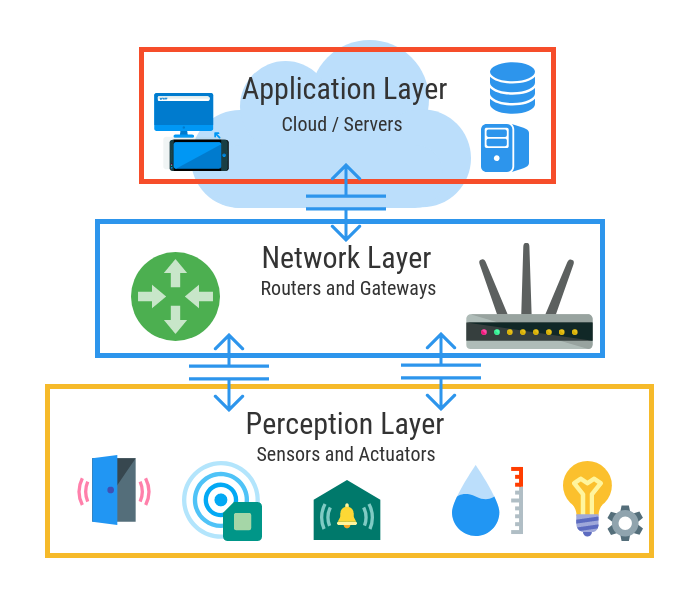
\includegraphics[width=\linewidth]{imagenes/arch-3-layer.png}
    \caption{Arquitectura de 3 capas}
    \label{fig:figure1}
\end{figure}

\newpage


\subsection{Protocolos}



\subsection{Tecnologías asociadas}


\subsection{Retos}



\section{Seguridad}

\subsection{Aspectos legales y éticos}


\subsection{Privacidad}


\subsection{Auditoría de seguridad}


\subsection{Seguridad de datos}

}